% !TeX root = ./main.tex

\chapter*{\large ПРИЛОЖЕНИЕ А\\Презентация к защите реферата (15 слайдов)}
\addcontentsline{toc}{chapter}{ПРИЛОЖЕНИЕ А Презентация к защите реферата}

Полная презентация сохранена в файле \nolinkurl{Certified_Cross-Scale_Graph_Morphometry.pdf}. Ниже приведены все 15~слайдов доклада.

\vspace{0.3cm}
\noindent
\begin{tabularx}{\textwidth}{@{} C C @{}}
    \fbox{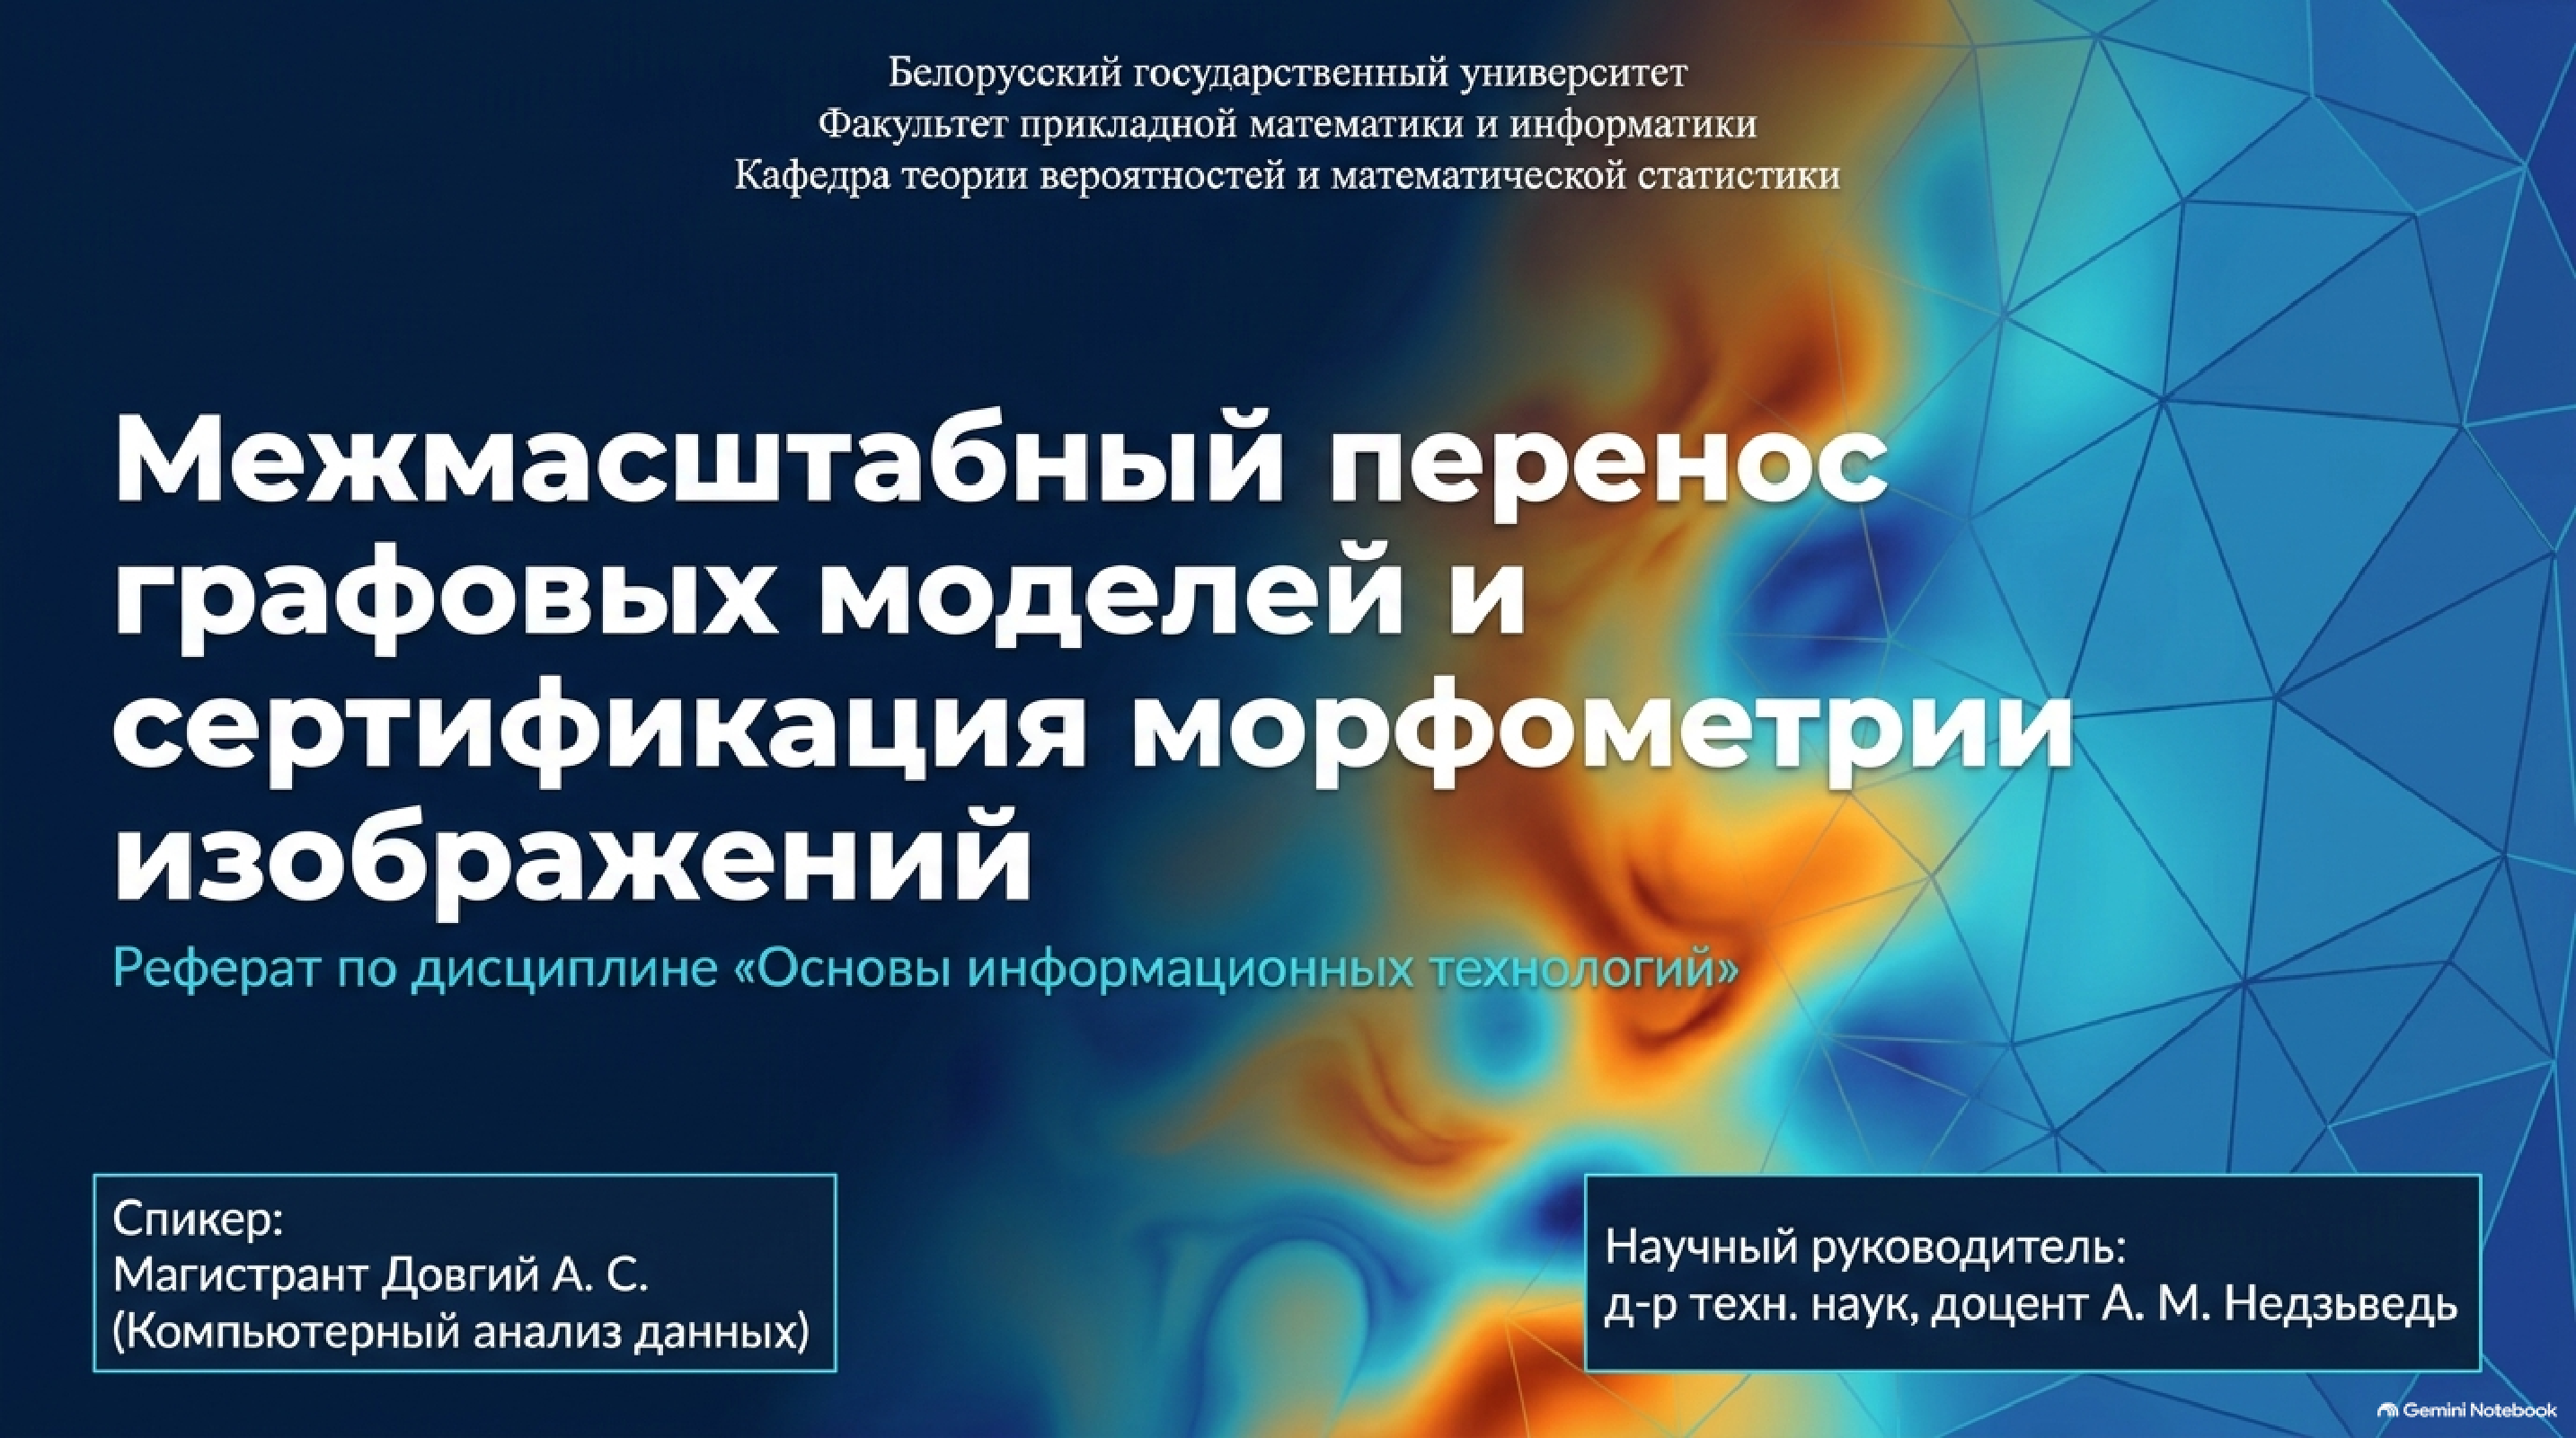
\includegraphics[page=1, width=0.46\textwidth]{../Certified_Cross-Scale_Graph_Morphometry.pdf}} &
    \fbox{\includegraphics[page=2, width=0.46\textwidth]{../Certified_Cross-Scale_Graph_Morphometry.pdf}} \\[0.35cm]
    \fbox{\includegraphics[page=3, width=0.46\textwidth]{../Certified_Cross-Scale_Graph_Morphometry.pdf}} &
    \fbox{\includegraphics[page=4, width=0.46\textwidth]{../Certified_Cross-Scale_Graph_Morphometry.pdf}} \\[0.35cm]
    \fbox{\includegraphics[page=5, width=0.46\textwidth]{../Certified_Cross-Scale_Graph_Morphometry.pdf}} &
    \fbox{\includegraphics[page=6, width=0.46\textwidth]{../Certified_Cross-Scale_Graph_Morphometry.pdf}}
\end{tabularx}

\newpage
\noindent
\begin{tabularx}{\textwidth}{@{} C C @{}}
    \fbox{\includegraphics[page=7, width=0.46\textwidth]{../Certified_Cross-Scale_Graph_Morphometry.pdf}} &
    \fbox{\includegraphics[page=8, width=0.46\textwidth]{../Certified_Cross-Scale_Graph_Morphometry.pdf}} \\[0.35cm]
    \fbox{\includegraphics[page=9, width=0.46\textwidth]{../Certified_Cross-Scale_Graph_Morphometry.pdf}} &
    \fbox{\includegraphics[page=10, width=0.46\textwidth]{../Certified_Cross-Scale_Graph_Morphometry.pdf}} \\[0.35cm]
    \fbox{\includegraphics[page=11, width=0.46\textwidth]{../Certified_Cross-Scale_Graph_Morphometry.pdf}} &
    \fbox{\includegraphics[page=12, width=0.46\textwidth]{../Certified_Cross-Scale_Graph_Morphometry.pdf}}
\end{tabularx}

\newpage
\noindent
\begin{tabularx}{\textwidth}{@{} C C @{}}
    \fbox{\includegraphics[page=13, width=0.46\textwidth]{../Certified_Cross-Scale_Graph_Morphometry.pdf}} &
    \fbox{\includegraphics[page=14, width=0.46\textwidth]{../Certified_Cross-Scale_Graph_Morphometry.pdf}}
\end{tabularx}

\vspace{0.35cm}
\begin{center}
    \fbox{\includegraphics[page=15, width=0.46\textwidth]{../Certified_Cross-Scale_Graph_Morphometry.pdf}}
\end{center}

\newpage

\chapter*{\large ПРИЛОЖЕНИЕ Б\\Персональный научный веб-ресурс и авторский программный комплекс}
\addcontentsline{toc}{chapter}{ПРИЛОЖЕНИЕ Б Персональный научный веб-ресурс и авторский программный комплекс}

Для открытого доступа к интерактивной презентации, документации по модулям программного комплекса \texttt{CDQuad}, таблицам верификации и исходным кодам расчётов развёрнут персональный научно-образовательный веб-ресурс соискателя на платформе GitHub Pages: \url{https://ihuod.github.io/BSU-FIT/}. Векторный макет интерфейса главной страницы ресурса приведён ниже.

\begin{figure}[htbp]
\centering
\resizebox{0.96\textwidth}{!}{%
\begin{tikzpicture}[font=\sffamily]
    % Окно браузера
    \draw[rounded corners=6pt, fill=bsuSoft, draw=bsuBlue!50, line width=1pt] (0,0) rectangle (16,9.2);
    \fill[bsuBlue!15] (0,8.4) rectangle (16,9.2);
    \fill[red!70] (0.5,8.8) circle (0.13);
    \fill[orange!80] (0.95,8.8) circle (0.13);
    \fill[green!65!black] (1.4,8.8) circle (0.13);
    \draw[rounded corners=3pt, fill=white, draw=bsuBlue!30] (2.2,8.55) rectangle (14.5,9.05);
    \node[font=\scriptsize\ttfamily, text=bsuBlue] at (8.35,8.8) {https://ihuod.github.io/BSU-FIT/};

    % Шапка сайта
    \fill[bsuBlue] (0,6.3) rectangle (16,8.4);
    \node[font=\normalsize\bfseries\sffamily, text=white] at (8,7.75) {Межмасштабный перенос графовых моделей и сертификация морфометрии};
    \node[font=\sffamily\scriptsize, text=white!90] at (8,7.15) {Программный комплекс CDQuad $\bullet$ Магистрант ФПМИ БГУ Довгий А.~С.};
    \node[font=\scriptsize, text=bsuSoft] at (8,6.65) {Кафедра ТВиМС $\bullet$ Научный руководитель: д-р техн. наук, доц. А.~М.~Недзьведь};

    % 4 карточки ключевых метрик
    \foreach \x/\val/\cap in {
        0.4/2{,}28$\times$/Снижение ошибки поля на 54$\times$54,
        4.3/$r=0{,}9803$/Корреляция дефекта $\widehat{\delta}_{-1}(G)$,
        8.2/$-36{,}1\,\%$/Сужение 90\,\% конформного интервала,
        12.1/4{,}1--4{,}4$\times$/Снижение дрейфа на живой клетке
    }{
        \draw[rounded corners=4pt, fill=white, draw=bsuAccent, line width=0.8pt] (\x,4.2) rectangle (\x+3.5,5.95);
        \node[font=\small\bfseries, text=bsuBlue] at (\x+1.75,5.4) {\val};
        \node[font=\tiny, text=black!80, text width=3.2cm, align=center] at (\x+1.75,4.68) {\cap};
    }

    % Блоки описания архитектуры и публикаций
    \draw[rounded corners=4pt, fill=white, draw=bsuBlue!30] (0.4,2.2) rectangle (15.6,3.85);
    \node[anchor=west, font=\footnotesize\bfseries, text=bsuBlue] at (0.7,3.48) {Модульная архитектура открытого пакета и интерактивный просмотрщик слайдов};
    \node[anchor=west, font=\scriptsize, text width=14.6cm] at (0.7,2.75) {
        $\bullet$ \texttt{src/meshes.py} -- сетки Делоне, ячейки Дональда, SLIC RAG \quad
        $\bullet$ \texttt{src/operators.py} -- $P_1$-жёсткость $K(x)$ и потоки $F_{ij}$\\
        $\bullet$ \texttt{src/certificate.py} -- двойственный дефект $H_G^{-1}$ и split CP \quad
        $\bullet$ \texttt{src/descriptors.py} -- липшицева морфометрия изображений
    };

    \draw[rounded corners=4pt, fill=white, draw=bsuBlue!30] (0.4,0.35) rectangle (15.6,1.9);
    \node[anchor=west, font=\footnotesize\bfseries, text=bsuBlue] at (0.7,1.52) {Научные публикации и открытый репозиторий GitHub (\texttt{ihuod/BSU-FIT})};
    \node[anchor=west, font=\scriptsize, text width=14.6cm] at (0.7,0.85) {
        $\bullet$ Вестник БГУ. Сер.~1 (2026) $\bullet$ BIG DATA and Advanced Analytics (БГУИР, 2026, с.~319--329) $\bullet$ 83-я конф. БГУ\\
        $\bullet$ Реферат PDF, презентация (15 слайдов) и протоколы \texttt{results/exp1..exp3\_results.json} в открытом доступе
    };
\end{tikzpicture}%
}
\caption{Векторный макет главной страницы персонального научно-образовательного веб-ресурса проекта \texttt{CDQuad}}
\label{fig:site_mockup}
\end{figure}

\vspace{0.3cm}
\noindent
\begin{minipage}[c]{0.22\textwidth}
    \centering
    
\includegraphics[width=3.0cm]{figures/qr_code.pdf}
\end{minipage}\hfill
\begin{minipage}[c]{0.75\textwidth}
    {\small\textbf{Реквизиты открытого программного комплекса соискателя:}}\par\vspace{3pt}
    {\footnotesize\raggedright
    $\bullet$ Веб-ресурс (GitHub Pages): \url{https://ihuod.github.io/BSU-FIT/}\par
    $\bullet$ Репозиторий исходного кода: \url{https://github.com/ihuod/BSU-FIT}\par
    $\bullet$ Вычислительное ядро: \texttt{src/meshes.py}, \texttt{src/operators.py}, \texttt{src/certificate.py}, \texttt{src/descriptors.py}\par
    $\bullet$ Лицензия распространения: открытая лицензия MIT.\par}
\end{minipage}
